%============================================================
\section{Introduction}
%============================================================
Clinical diagnosis is inherently multimodal: a radiologist reads a chest radiograph in the
context of the presenting complaint, the history, vital signs and laboratory results.
Deep-learning systems that mirror this practice have moved from \emph{non-unified} pipelines,
in which each modality is encoded separately and combined only at the decision level, towards
\emph{unified} transformers that tokenise every modality and let attention mix them
\citep{huang2020fusion,acosta2022multimodal,xu2023mmtsurvey}. IRENE \citep{zhou2023irene} is a
representative clinical instance: chest X-ray patches, chief-complaint tokens, demographics and
laboratory values are all embedded as tokens; the first two layers apply \emph{bidirectional
multimodal attention}, in which the image stream and the clinical stream each attend to
themselves and to the other stream, and the remaining layers perform joint self-attention over
the concatenated sequence.

Three design decisions in such models are rarely isolated experimentally:
(i)~\textbf{where} to fuse (early, mid, or late);
(ii)~\textbf{how} the streams exchange information (bidirectional, unidirectional, co-attention,
gated cross-attention); and
(iii)~whether an explicit \textbf{image--text alignment} objective in a shared embedding space
(CLIP \citep{radford2021clip}, SigLIP \citep{zhai2023siglip}), which dominates 2023--2024
vision--language pre-training \citep{li2023blip2,girdhar2023imagebind,zhang2023biomedclip,you2023cxrclip},
also helps a supervised clinical fusion model. The original IRENE was trained on a private
cohort, so these questions cannot be revisited on its data. This paper does so on a fully public
dataset.

\paragraph{Contributions.}
\begin{itemize}
\item An open, reproducible re-implementation of IRENE for a public multimodal chest-radiograph
dataset \citep{cohen2020covid}, including an image--text--structured data pipeline
(cleaning, de-identification of dates, label-leakage masking, missing-value encoding and
patient-grouped splits) and a modernised training stack (native AMP, DDP, tuned
\texttt{DataLoader}, W\&B tracking) that replaces the original apex/\texttt{DataParallel} code.
\item A single configurable architecture, IRENE-MM, that expresses early, mid and late fusion,
six cross-modal attention structures and two contrastive objectives as switches, so that
ablations differ in exactly one factor.
\item A controlled study over \NRuns{} configurations with 5-fold patient-grouped cross-validation
and multiple seeds, reporting pooled out-of-fold macro AUROC with patient-level bootstrap
confidence intervals, missing-modality robustness and cross-modal retrieval.
\item Evidence that free-text notes in public COVID-19 collections leak the label, which, if
unmasked, inflates text-based and fused models (a multimodal counterpart of the shortcut
learning documented for radiographs \citep{degrave2021shortcuts,roberts2021pitfalls}).
\end{itemize}

%============================================================
\section{Related work}
%============================================================
\paragraph{Fusion in clinical multimodal models.}
Surveys distinguish early (input/feature-level), joint/intermediate and late (decision-level)
fusion \citep{huang2020fusion,acosta2022multimodal}. MedFuse \citep{hayat2022medfuse} combines
chest X-rays with clinical time series through an LSTM fusion module robust to missing inputs;
IRENE \citep{zhou2023irene} uses a unified transformer with bidirectional multimodal attention
followed by joint self-attention. In general vision--language models, single-stream
(``merged attention'') and dual-stream co-attention designs such as ViLBERT and LXMERT
\citep{lu2019vilbert,tan2019lxmert} represent the two ends of the spectrum; attention
bottlenecks \citep{nagrani2021bottleneck} showed that restricting cross-modal flow to later
layers can improve accuracy and cost, and Flamingo \citep{alayrac2022flamingo} introduced
tanh-gated cross-attention layers inserted into frozen backbones. Ma et al.\ \citep{ma2022missing}
showed that multimodal transformers are fragile when a modality is missing at test time and that
the optimal fusion strategy is dataset-dependent.

\paragraph{Image--text alignment.}
CLIP \citep{radford2021clip} learns a shared embedding space with a symmetric InfoNCE loss
\citep{oord2018cpc}; SigLIP \citep{zhai2023siglip} replaces the softmax with a pairwise sigmoid
loss that does not require global normalisation. ALBEF \citep{li2021albef} and BLIP-2
\citep{li2023blip2} align unimodal representations \emph{before} fusing them with cross-attention.
ImageBind \citep{girdhar2023imagebind} binds many modalities into one space through image-paired
data. In medicine, ConVIRT \citep{zhang2022convirt}, GLoRIA \citep{huang2021gloria},
MedCLIP \citep{wang2022medclip}, MGCA \citep{wang2022mgca}, MedKLIP \citep{wu2023medklip},
CXR-CLIP \citep{you2023cxrclip} and BiomedCLIP \citep{zhang2023biomedclip} pre-train
radiograph--report encoders contrastively, and generalist models such as LLaVA-Med
\citep{li2023llavamed} and Med-PaLM~M \citep{tu2024medpalmm} extend this to instruction following.
We study the contrastive objective not as pre-training on millions of pairs but as an auxiliary
loss inside a small supervised fusion model, the regime of most hospital-scale datasets.

\paragraph{Shortcuts in COVID-19 imaging.}
DeGrave et al.\ \citep{degrave2021shortcuts} and Roberts et al.\ \citep{roberts2021pitfalls}
showed that many COVID-19 radiograph classifiers exploit dataset artefacts. We add that
\emph{text} in public case collections carries even more direct shortcuts: diagnosis and
pathogen names.

%============================================================
\section{Data}
\label{sec:data}
%============================================================
\paragraph{Source.} We use the COVID-19 Image Data Collection \citep{cohen2020covid}
(\url{https://github.com/ieee8023/covid-chestxray-dataset}), a public set of cases compiled from
publications and case repositories. Each image has metadata that naturally splits into
IRENE's three input types: the radiograph, an unstructured \texttt{clinical\_notes} field
(the presenting history and imaging findings, written by many authors in many
institutions; several are machine translations of non-English case reports),
and structured fields (age, sex, days since symptom onset, temperature,
SpO$_2$, leukocyte, neutrophil and lymphocyte counts, and the radiographic view).
\Cref{fig:dataset} summarises the processed data.

\paragraph{Cohort and labels.} From \RawRows{} rows we keep the \XrayRows{} radiographs,
drop \texttt{todo}/\texttt{Unknown} findings, and obtain \NImages{} images from \NPatients{}
patients. The hierarchical \texttt{finding} string (e.g.\ \texttt{Pneumonia/Viral/COVID-19})
is mapped to 7 targets: COVID-19, other viral, bacterial, fungal, other/unspecified pneumonia
(including lipoid and aspiration), tuberculosis, and no finding. Classes are highly imbalanced
(\cref{fig:dataset}a); following IRENE the model is trained with multi-label binary
cross-entropy and evaluated with per-class and macro AUROC.

\paragraph{Text processing.} Notes are Unicode-normalised (NFKC), stripped of URLs and
figure/panel references, whitespace-normalised, and dates are replaced by a \texttt{[DATE]}
token (\DateNotes{} notes contain a date). Crucially, \NotesMasked{} of the \NotesWith{} notes
(\PctMasked\%) contain the diagnosis or pathogen by name (``COVID-19'', ``SARS-CoV-2'',
``\emph{Pneumocystis}'', ``tuberculosis'', \dots). Unless stated otherwise we replace
\NMaskedTerms{} such terms by a \texttt{[DX]} token; \cref{sec:leak} quantifies the effect of
not doing so. Notes are tokenised with spaCy \citep{honnibal2020spacy}; each token is
represented by a 300-d static word vector plus three indicator channels
(\texttt{[DX]}, \texttt{[DATE]}, out-of-vocabulary), mirroring IRENE's per-token text features.

\paragraph{Structured data.} Continuous fields are robustly standardised (median/IQR, clipped
to $\pm5$) and each value carries an observation mask: laboratory values are missing for
over 95\% of images (\cref{fig:dataset}c). The view (PA/AP/AP supine/lateral) is one-hot encoded.
RT-PCR status and outcomes (survival, ICU, intubation) are excluded because they reveal or
post-date the label.

\paragraph{Splits.} Many patients contribute several images (up to 8), often with the same
note. We therefore use 5-fold \emph{patient-grouped}, label-stratified cross-validation
(\texttt{StratifiedGroupKFold}); within each training fold 15\% of patients are held out
for early stopping. All numbers are computed on out-of-fold (OOF) predictions pooled over the
five test folds (\NImages{} images), which avoids unstable AUROCs for classes with 3--4
positives per fold.

\begin{figure*}[t]
\centering
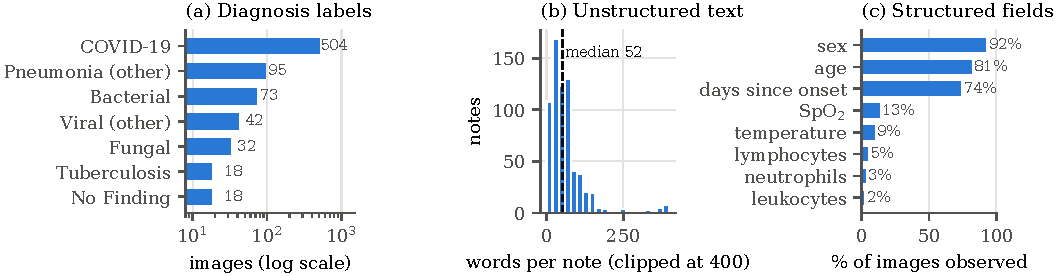
\includegraphics[width=\textwidth]{figures/dataset.pdf}
\caption{Processed dataset. (a) Label counts (log scale). (b) Length of the unstructured
clinical notes (\NotesWith{} of \NImages{} images have one). (c) Fraction of images for which
each structured field is observed; missing values are encoded with learned missing-value
embeddings rather than imputed.}
\label{fig:dataset}
\end{figure*}

%============================================================
\section{Method}
\label{sec:method}
%============================================================
\begin{figure*}[t]
\centering
\resizebox{0.96\textwidth}{!}{% IRENE-MM architecture (TikZ). Included from main.tex.
\begin{tikzpicture}[
  font=\scriptsize,
  box/.style={draw=black!70, rounded corners=2pt, minimum height=0.55cm, align=center, inner sep=2pt},
  tok/.style={draw=black!60, minimum width=0.16cm, minimum height=0.32cm, inner sep=0pt},
  arr/.style={-{Stealth[length=1.6mm]}, black!70, line width=0.5pt},
  lab/.style={font=\scriptsize\itshape, text=black!65},
]
% ---------------- inputs
\node[box, fill=blue!6, minimum width=1.9cm] (img) at (0,0) {chest X-ray\\224$\times$224};
\node[box, fill=orange!8, minimum width=1.9cm] (txt) at (0,-1.5) {clinical note\\([DX]-masked)};
\node[box, fill=green!7, minimum width=1.9cm] (tab) at (0,-2.75) {age, sex, vitals,\\labs, view (+mask)};

% ---------------- tokenisers
\node[box, fill=blue!6, minimum width=2.0cm] (cnn) at (2.55,0) {frozen CXR\\DenseNet-121};
\node[box, fill=orange!8, minimum width=2.0cm] (wv) at (2.55,-1.5) {tokenise +\\word vectors};
\node[box, fill=green!7, minimum width=2.0cm] (lin) at (2.55,-2.75) {Linear(1$\to$d)\\+ missing emb.};
\draw[arr] (img) -- (cnn); \draw[arr] (txt) -- (wv); \draw[arr] (tab) -- (lin);

% token strips
\foreach \i in {0,...,5} {\node[tok, fill=blue!25] at (4.1+\i*0.19,0) {};}
\foreach \i in {0,...,5} {\node[tok, fill=orange!35] at (4.1+\i*0.19,-1.5) {};}
\foreach \i in {0,...,5} {\node[tok, fill=green!35] at (4.1+\i*0.19,-2.75) {};}
\node[lab] at (4.58,0.38) {image tokens $\mathbf{X}_I$};
\node[lab] at (4.58,-1.12) {note tokens};
\node[lab] at (4.58,-3.13) {structured tokens};
\draw[arr] (cnn) -- (3.98,0); \draw[arr] (wv) -- (3.98,-1.5); \draw[arr] (lin) -- (3.98,-2.75);
\draw[decorate, decoration={brace, amplitude=3pt, mirror}, black!60] (5.25,-3.0) -- (5.25,-1.3)
  node[midway, right=1pt, lab, align=left, font=\tiny\itshape] {clinical\\stream $\mathbf{X}_C$};

% ---------------- dual-stream blocks
\node[box, fill=black!4, minimum width=2.9cm, minimum height=3.35cm] (dual) at (8.3,-1.2) {};
\node[font=\scriptsize\bfseries, fill=black!4] at (8.3,0.2) {$k\times$ dual-stream block};
\node[box, fill=blue!10, minimum width=0.95cm] (si) at (7.55,-0.3) {Self$_I$};
\node[box, fill=orange!12, minimum width=0.9cm] (sc) at (7.55,-2.1) {Self$_C$};
\node[box, fill=purple!10, minimum width=1.2cm] (ci) at (9.0,-0.3) {Cross$_{I\leftarrow C}$};
\node[box, fill=purple!10, minimum width=1.2cm] (cc) at (9.0,-2.1) {Cross$_{C\leftarrow I}$};
\draw[arr, purple!60, densely dashed] (8.85,-1.8) -- (8.85,-0.62);
\draw[arr, purple!60, densely dashed] (9.15,-0.62) -- (9.15,-1.8);
\node[lab, align=center, font=\tiny] at (7.75,-1.2) {combine by\\\texttt{cross\_mode}};
\draw[arr] (5.3,0) -- (7.0,-0.3);
\draw[arr] (6.35,-2.1) -- (7.0,-2.1);

% ---------------- alignment
\node[box, fill=teal!8, minimum width=1.75cm] (align) at (8.3,-3.75) {CLIP / SigLIP\\$\mathcal{L}_{\text{align}}$ on $z_I, z_T$};
\draw[arr, teal!70!black] (8.3,-2.88) -- (align);
\node[lab, font=\tiny, align=right, anchor=east] at (6.9,-3.75) {unimodal pass\\(cross disabled)};

% ---------------- joint blocks
\node[box, fill=black!4, minimum width=1.6cm, minimum height=1.5cm, align=center] (joint) at (11.35,-1.2) {$(L{-}k)\times$\\joint self-\\attention\\on $[\mathbf{X}_I;\mathbf{X}_C]$};
\draw[arr] (9.75,-0.3) -- (10.55,-0.9); \draw[arr] (9.75,-2.1) -- (10.55,-1.5);
\node[box, fill=red!6, minimum width=1.6cm] (head) at (11.35,-2.85) {masked mean\\pool + linear};
\draw[arr] (joint) -- (head);
\node[box, minimum width=1.6cm] (out) at (11.35,-3.9) {7 diagnoses\\$\mathcal{L}_{\text{BCE}}$};
\draw[arr] (head) -- (out);
\end{tikzpicture}
}
\caption{IRENE-MM. Each modality is tokenised; the image stream $\mathbf{X}_I$ and the clinical
stream $\mathbf{X}_C$ (note + structured tokens) pass through $k$ dual-stream blocks whose
cross-modal exchange is set by \texttt{cross\_mode}, then through $L-k$ joint self-attention blocks.
$k=0$ is early fusion; $k=L$ with no cross-attention is late fusion; IRENE is $k=2$ with
bidirectional attention. The optional alignment loss is computed on \emph{unimodal}
pooled embeddings (a second pass through the dual-stream blocks with cross-attention
disabled), so that the note embedding cannot see the image.}
\label{fig:arch}
\end{figure*}

\paragraph{Tokenisation.} \Cref{fig:arch} shows the architecture. Following the ``hybrid''
tokeniser that IRENE inherits from ViT \citep{dosovitskiy2021vit}, radiographs are encoded by a
DenseNet-121 \citep{huang2017densenet} pretrained on seven public chest X-ray datasets
(\texttt{torchxrayvision} \texttt{densenet121-res224-all} \citep{cohen2022torchxrayvision}),
kept frozen; its $7{\times}7{\times}1024$ feature map is average-pooled to a $4{\times}4$ grid
and linearly projected to $d$-dimensional image tokens with learned position embeddings.
Five views per image (one clean, four randomly cropped, rotated and intensity-jittered) are
cached; training samples a random view per step. Note tokens (at most \MaxTxt{}) are linearly
projected; age and sex use IRENE's scalar embeddings \texttt{Linear(1,$d$)}, and each structured
value $v_j$ with mask $m_j$ becomes $m_j\,W v_j + (1-m_j)\,e^{\text{miss}}_j + p_j$ with a
shared projection $W$, a learned missing embedding and a position embedding.

\paragraph{Dual-stream block.} Let $h_I=\mathrm{LN}(\mathbf{X}_I)$, $h_C=\mathrm{LN}(\mathbf{X}_C)$,
$S_I=\mathrm{Attn}(h_I,h_I)$, $S_C=\mathrm{Attn}(h_C,h_C)$ and the cross terms
$X_{I\leftarrow C}=\mathrm{Attn}(q{=}h_I,kv{=}h_C)$, $X_{C\leftarrow I}=\mathrm{Attn}(q{=}h_C,kv{=}h_I)$,
each with its own projections and key-padding masks. The attention outputs $A_I, A_C$ are
\begin{center}
\small
\begin{tabular}{@{}lll@{}}
\toprule
\texttt{cross\_mode} & $A_I$ & $A_C$ \\
\midrule
\texttt{bi\_avg} (IRENE) & $(S_I+X_{I\leftarrow C})/2$ & $(S_C+X_{C\leftarrow I})/2$\\
\texttt{bi\_cross} (co-attn.) & $X_{I\leftarrow C}$ & $X_{C\leftarrow I}$\\
\texttt{i2t} & $(S_I+X_{I\leftarrow C})/2$ & $S_C$\\
\texttt{t2i} & $S_I$ & $(S_C+X_{C\leftarrow I})/2$\\
\texttt{gated} & $S_I+\tanh(\alpha_I)X_{I\leftarrow C}$ & $S_C+\tanh(\alpha_C)X_{C\leftarrow I}$\\
\texttt{none} & $S_I$ & $S_C$\\
\bottomrule
\end{tabular}
\end{center}
followed by per-stream output projections, residual connections and feed-forward networks.
\texttt{bi\_avg} is IRENE's equation (averaging self- and cross-attention contexts);
\texttt{bi\_cross} corresponds to ViLBERT/LXMERT co-attention \citep{lu2019vilbert,tan2019lxmert};
\texttt{gated} follows Flamingo's zero-initialised tanh gates \citep{alayrac2022flamingo}.

\paragraph{Fusion position.} After $k$ dual-stream blocks the streams are concatenated and
processed by $L-k$ standard pre-LN blocks \citep{vaswani2017attention}. The prediction is a
linear head on the masked mean of all tokens (IRENE also mean-pools). With $k=0$ the model is a
single-stream early-fusion transformer; with $k=L$ and \texttt{none} the streams never interact
and their pooled features are concatenated before the head (late fusion).

\paragraph{Contrastive alignment.} With projection heads $g_I,g_T$ and pooled unimodal
embeddings $z_I, z_T$ (image tokens; note tokens only), the auxiliary loss is either
CLIP/InfoNCE \citep{radford2021clip},
$\mathcal{L}=\tfrac12\big[\mathrm{CE}(\tau S, Y)+\mathrm{CE}(\tau S^\top, Y^\top)\big]$,
or SigLIP \citep{zhai2023siglip},
$\mathcal{L}=-\tfrac1B\sum_{ij}\log\sigma\big(y_{ij}(\tau S_{ij}+b)\big)$, where
$S_{ij}=g_I(z_I^i)^\top g_T(z_T^j)$ on $\ell_2$-normalised vectors and $\tau$ (and $b$) are learned.
Because images of the same patient often share one note, $Y$ marks \emph{all} pairs with
identical notes as positives (multi-positive targets) instead of treating them as negatives.
Following ALBEF \citep{li2021albef} we align before fusing; unlike a naive implementation that
pools the text stream after cross-attention---where the text embedding already contains the
image and retrieval becomes trivial (we observed R@1 $>0.8$ in a pilot)---$z_I,z_T$ come from a
weight-shared pass through the dual-stream blocks with cross-attention switched off.
The total loss is $\mathcal{L}_{\text{BCE}}+\lambda\mathcal{L}_{\text{align}}$.

\paragraph{Missing modalities.} All attention uses key-padding masks, so images without a note
simply have no note tokens. We evaluate every model a second time with the note removed at test
time, and optionally train with \emph{modality dropout} (note removed with probability 0.3).

%============================================================
\section{Experimental setup}
\label{sec:setup}
%============================================================
\paragraph{Model and training.} All variants use $L{=}6$ layers, $d{=}128$, 4 heads and an MLP
width of 256 (\ParamMin--\ParamMax\,M trainable parameters depending on the variant; the frozen DenseNet
is not counted), dropout 0.1. We train with AdamW \citep{loshchilov2019adamw}
(lr $3{\times}10^{-4}$, weight decay 0.05, one-cycle schedule), batch size 32, gradient clipping 1.0,
at most 25 epochs with early stopping on the validation BCE (patience 5), restoring the best
checkpoint. The contrastive projection dimension is 128.

\paragraph{Protocol.} Every configuration is run on the same five folds with \NSeedsMain{} seeds
(main comparison) or 2 seeds (ablations). We report pooled-OOF macro AUROC (mean $\pm$ s.d.\ over
seeds), macro AUPRC, macro F1 and accuracy of the arg-max prediction, a 95\% patient-level
bootstrap interval of the seed-averaged OOF predictions (1{,}000 resamples), and paired
patient-level bootstrap tests between models. Cross-modal retrieval is image$\to$note Recall@$K$
within each test fold (gallery = distinct notes in the fold, $\approx$120), averaged over folds.

\paragraph{Engineering.} The training stack (\texttt{train.py}) uses PyTorch \citep{paszke2019pytorch}
\texttt{DataLoader} workers with pinned memory, persistent workers and prefetching; automatic mixed
precision \citep{micikevicius2018mixed} (fp16 with loss scaling on GPU, bf16 autocast on CPU);
\texttt{DistributedDataParallel} \citep{li2020ddp} launched with \texttt{torchrun}
(NCCL on GPU, Gloo on CPU) with a \texttt{DistributedSampler}; and Weights \& Biases
\citep{biewald2020wandb} logging of every epoch, fold and seed (offline mode; synchronisable with
\texttt{wandb sync}). All experiments in this paper were run on a 2-core CPU machine without a GPU;
\cref{sec:throughput} reports the throughput measurements we could make there.
